%!TEX root = ../main.tex
%%%%%%%%%%%%%%%%%%%%%%%%%%%%%%%%%%
% Links:
%
% Difficulty: Easy/Medium
% Companies: 
%%%%%%%%%%%%%%%%%%%%%%%%%%%%%%%%%%

\chapterimage{header}

\chapter{Power set generation}
\label{ch:power_set}
\section*{Introduction}


\section{Problem statement}
Write a function that given a collection $S$ returns its power-set. A power-set of a collection $S$ is the set of all its ordered subsets including the empty subset and S itself. Subsets can appear in any order.

\begin{example}
	\hfill \\
	For the collection of characters $S=\{a,b,c\}$  both $P$ and $P'$ are two valid outputs of the function:
	\begin{equation*}
		P = \{\{\}, \{b,c\}, \{a\}, \{a,b\}, \{a,b,c\}, \{b\}, \{a,c\}, \{c\} \}
	\end{equation*}
	\begin{equation*}
		P' = \{\{\}, \{a\}, \{b\}, \{c\}, \{a,b\}, \{b,c\}, \{a,c\}, \{a,b,c\} \}
	\end{equation*}
	
\end{example}

\section{Clarification Questions}

\begin{QandA}
	\item What is the maximum size of the input?
	\begin{answered}
		\textit{The maximum number of element is strictly less than $n < 32$.}
	\end{answered}
	
	\item Are all the element in the collection distinct?
	\begin{answered}
		\textit{No, the elements are not necessarily distinct. $S$ can contain duplicates.
}
	\end{answered}
\end{QandA}

\section{Discussion}
There is one key point that should immediately be noticed:
\begin{itemize}
	\item \textbf{The powerset of a collection of $n$ elements has size $2^n$}. This fact should be immediately pointed out during the interview, stressing the fact that the constraint $n < 32$ is a strong hint towards the fact that an exponential solution is expected. Doing so shows knowledge on powersets and the ability to link and use that knowledge with the problem statement.
\end{itemize}

\subsection{Backtracking}
The solution to this problem is based on the fact that that during the generation of one of the elements of the power-set a decision has to be taken, for each element of the original collection, on whether to include or not into the subset.
We thus have two choices for each element of the input and that can be easily visualized drawing a tree as shown in Figure \ref{ref:power_set_decision_trees}.

One general way to deal with such type of problems is by using backtracking to try all possible decision paths for each of the elements. The proposed solution will incrementally construct one subset at the time, using an integer variable to keep track of which element we are currently deciding to include or exclude.
The base case of the recursion happen when there is no more decision to take, meaning that the current subset is ready to be included in the solution (it has been produced after $n$ decision steps).
The C++ code implementing the idea above is shown in Listing \ref{list:power_set_backtracking}.
\lstinputlisting[language=c++, caption="C++ to the power set generation using backtracking",label=list:power_set_backtracking]{sources/power_set/power_set_backtracking.cpp}

\begin{figure}
	\label{ref:power_set_decision_trees}
	\centering
	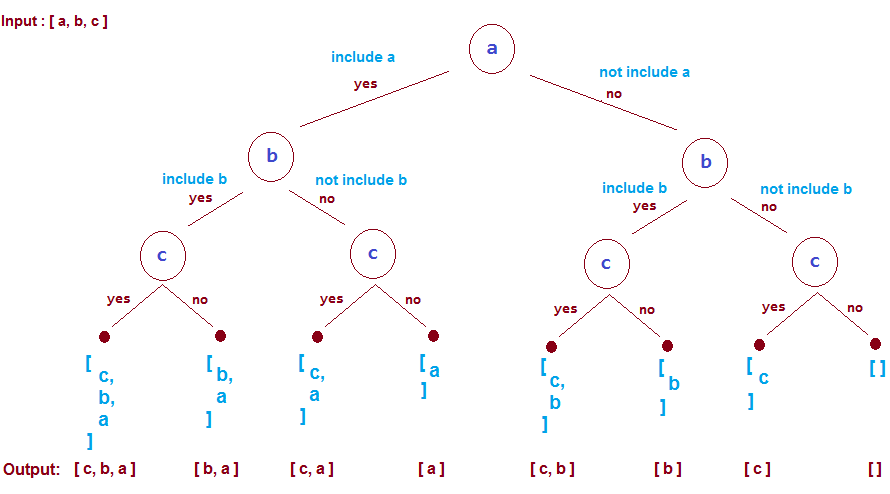
\includegraphics[scale=2.0]{sources/power_set/images/subsetTree}
	\caption{Decision tree for the power-set generation using backtracking.}
\end{figure}

The complexity of the backtrack solution is exponential i.e. $O(2^n)$ which is as good as it gets.

\subsection{Bit Manipulation}
Another approach that can be used to solve this problem is based on the fact that the values of the bits of the numbers $\{0,1,2,\ldots, s^n-1\}$  already provide all the information necessary to make decision weather to include or not an element from the input. In other words the set of numbers $P=\{0,1,2,\ldots, s^n-1\}$ is a powerset of $n$ bits. The binary representation of the numbers can be used to build one subset. For instance
given the input $S={a,b,c}$ the Table \ref{tab:mapping_value_bits} shows how numbers maps to their bit representation on how that can be used to construct one subset of the power-set of $S$. A $1$ means the corresponding element is taken, while a $0$ means it is excluded.

\begin{table}[H]
	\centering
	\begin{tabular}{|l|l|l|}
		\hline
		Value & Bits & Subset\\ \hline
		0     & 000  & $\{\}$\\ \hline
		1     & 001  & $\{c\}$\\ \hline
		2     & 010  & $\{b\}$\\ \hline
		3     & 011  & $\{b,c\}$\\ \hline
		4     & 100  & $\{a\}$\\ \hline
		5     & 101  & $\{a,c\}$\\ \hline
		6     & 110  & $\{a,b\}$\\ \hline
		7     & 111  & $\{a,b,c\}$\\ \hline
	\end{tabular}
	\label{tab:mapping_value_bits}
\end{table}

This idea can be used to write an algorithm in which all the numbers in the range $\{0,1,2,\ldots, s^n-1\}$ are considered and each of them maps to a subset of the final solution. 
The following code implements the idea above\footnote{Notice the usage of the \texttt{reserve} function that should be used in all those scenario when we already know the final size of the collection we are building. This saves times because avoids intermediate allocation and copy that must happen during the resize of the vector.}.

\begin{minipage}{\linewidth}
	\lstinputlisting[language=c++, caption="C++ to the power set generation using backtracking",label=list:power_set_backtracking]{sources/power_set/power_set_bit_manipulation.cpp}
\end{minipage}

\section{Common variations}

\section{Conclusion}
